%Cyber physical systems - different than traditional embedded systems that interact with real world. Timing requirements, but large, and safety critical
\section{Motivation}
\emph{Cyber-Physical Systems} (CPS) are integrations of computation with physical processes~\todo{cite}.
In these systems, computation and physical process often form a tight feedback loop, affecting the behavior of each other.
The embedded platforms and networks employed not only control the physical process, but at the same time monitor and adapt to the changes of the physical process.
An enormous amount of applications can benefit from the potential of CPS.
They include high confidence medical devices and systems, assisted living, traffic control and safety, advanced automotive systems, process control, energy conservation, environmental control, avionics, instrumentation, critical infrastructure control (electric power, water resources, and communications systems for example), distributed robotics (telepresence, telemedicine), defense systems, manufacturing, and smart structures.
However, in order for CPS to be deployed in high confidence systems, such as advanced automotive or avionics systems, the platforms employed need to deal with two important properties of the physical process: they are inherently concurrent, and time progresses at its own pace.
 
%modern design techniques are hitting a scalability wall - RTOS, compilers, general purpose architectures all create problems
%all layers need work. Modern abstraction layers omit time.. designers need to reach down below, can't certify a system with its hardware
% We deal with the ISA and architecture design

Traditionally, real-time embedded systems have dealt with the notion of time.
These systems impose deadlines and timing constraints to its underlying tasks to deliver services in real time. 
The timing constraints of \emph{soft real-time systems} are typically used guarantee quality of service, while the constraints of \emph{hard real-time systems} are used to guarantee safety critical tasks, so they must be met. 
The real-time embedded community has widely adopted techniques proposed for general purpose applications, believing that they will provide the same advantages and benefits for embedded systems.
These include the programing language, the operating system, the tool-chains, and the computer architecture.
However, these techniques are designed for general purpose systems that do not require stringent interaction with the physical environment. 
Thus, they emphasize on improving average performance over predictability.   
As a result, when computing systems absolutely must meet tight timing constraints, these recent computing advances often do more harm than good~\cite{LeeOnTime2005}.
%this is contrary to reality~\cite{halang:DSP:2004:4,thiele_et_al:DSP:2004:2}.
The scale and complexity of traditional embedded systems allowed designers to compensate with extra effort in design and analysis. 
However, these solutions begin to break down when transitioning to CPS.   

In the current state of embedded software, nearly every abstraction has abstracted away \emph{time}.
The Instruction Set Architecture (ISA), meant to hide the hardware implementation details from the software, does not include a timing semantic for the instruction executions.  
Widely adopted programming languages, meant to hide the details of the ISA from the program logic, do not express timing properties; timing is merely an accident of the implementation.
Real-time operating systems (RTOS), meant to hide the details of the program from their concurrent orchestration, often use priorities to dictate the execution of tasks; the execution time of tasks can easily affect the scheduled outcome of execution.
The lack of \emph{time} in the abstraction layers lead to the following consequences:
\begin{itemize}
\item \emph{Unnecessary complexities in the interaction of concurrent components} --  
This often is manifested when components share resources. 
For example, software threads are the typical abstractions for concurrent software written in C or Java. 
Because there is no guarantee of when a shared variable will be accessed by each thread, locks and semaphores are required to avoid race conditions. 
This not only introduces bugs, but also introduces complex and almost impossible to analyze interactions between threads~\cite{Lee2006threads}. 
As a result, there is great difficulty when synchronizing and communicating between components or tasks.

\item \emph{Unnecessary complexities in interactions across layers} -- 
For example, scheduling could be done at multiple levels simultaneously without any coordination. 
As tasks or software threads are scheduled for execution in the OS, an explicit multithreaded dynamic dispatch architecture could also be scheduling instructions from different hardware threads without the knowledge of the OS~\cite{thiele_et_al:DSP:2004:2}.

\item \emph{Misleading or pessimistic analysis results when analyzing the whole system} -- 
For example, task scheduling and context switching cost may vary from the cache or pipeline state change after executing each tasks. 
This is often not factored into the analysis~\cite{thiele_et_al:DSP:2004:2}. 
Furthermore, because the  large variation of execution time in modern complex processors, WCET analysis techniques often lead to overly conservative results for safety~\cite{Wilhelm2008survey}. 
As the WCET is often the basis for priority of any scheduling scheme, the conservativeness is propagated throughout the system.
\end{itemize}
%explain composability

When the temporal properties of the system must be guaranteed, designers must reach beneath the abstraction layers, and understand thoroughly the complex underlying details and its affect on execution time. 
This not only increases the design complexity and effort, but the designed systems are \emph{brittle} and extremely sensitive to change~\cite{Sangiovanni-Vincentelli2007automotive, Edwards2007PRETcase}.  
For example, Sangiovanni-Vincentelli et al.\cite{Sangiovanni-Vincentelli2007automotive} showed that when increasing the execution time of a task, any priority based scheduling scheme results in discontinuity in the timing of all tasks besides the task with the highest priority. 
At a lower level, adding a few instructions can easily result in a huge variation in program execution time; the state of the hardware dynamic prediction and speculation units, such as caches and pipelines, can easily be affected by the minimum program additions, causing misprediction penalties.
Thus, in order to verify the timing of safety critical systems, the verification must be done on both the software system and its execution platform, they cannot be separated. 
This process is often time consuming and expensive.
Since the abstraction layers do not give any temporal semantics to the system, each layer must be completely understood in order to reason and prove the timing properties of the full system.  
For avionics manufactures, this means stockpiling the same hardware for the lifetime of an aircraft; any upgrade of components or software in their system could result in drastic timing changes, and thus require re-certification.


\subsection{Timing Predictable Systems}
Thiele et al.~\cite{thiele_et_al:DSP:2004:2}, Henzinger~\cite{Henzinger2008} and Lee~\cite{LeeOnTime2005} have all identified the importance and difficulties of designing \emph{timing-predictable systems}.
Timing-predictable systems should exhibit the following property: \textit{a small change in the input must not result in a large change in the output}~\cite{Henzinger2008}.
If the definition of \emph{output} includes the timing behavior exhibited by the system, then current abstracts disrupts this property at almost all levels. 

A change is needed to efficiently and safely design next generation systems, especially if they effect the well being of our lives.
In particular, how software and hardware deal with the notion of \textit{time} needs to be more carefully understood and designed.
At the lowest levels of abstraction, circuits and microarchitectures, timing is central to correctness.
For example, in a microarchitecture, if the output of an ALU is latched at the wrong time, the ISA will not be correctly implemented.
However, at higher levels, for example, the ISA, timing is hidden, and there is no temporal semantics; the execution time is irrelevant to correctness. 
Thus, each abstraction layer needs to be revisited to judiciously introduce some form of temporal semantics. 
Specifically for CPS, platforms must to be equip to handle the \emph{inherent concurrency} and the \emph{inexorable passage of time} for physical processes.   
Sangiovanni-Vincentelli et al.~\cite{Sangiovanni-Vincentelli2007automotive} identified these issues as the \textit{timing composability} and \textit{timing predictability} of systems, and lists them as requirements to enable efficient designs of large-scale safety-critical applications.    

\subsubsection{Timing Composability}
Modern systems handle the concurrency of physical processes with multiple tasks, components or subsystems that are integrated together.    
In order to efficiently design the system, these individual parts are designed and tested separately, then later integrated to form the final system. 
This modularity of design is crucial for the continued scaling and improvement of systems.      
However, if component properties may be destroyed during integration, then the components can no longer be designed and verified separately. 
\textit{Timing composability} refers to the ability to integrate components while preserving their temporal properties.

To preserve component properties during integration, modern designs often use a \textit{federated architecture}.
A Federated Architecture develops functions and features on physically separate platforms which are later integrated through an interconnect or system bus. 
As these features are only loosely coupled through an interconnect, interference is limited, allowing the preservation of certain properties independently verified. 
However, as each platform is feature specific, they are often idle during run time.
In order to reduce resource consumption, there is a shift towards \textit{integrated architectures}~\cite{Obermaisser2009FedtoIMA,AvionicsWatkins2007IMA}, where multiple functions are integrated on a single, shared platform.
Several challenges exists during this shift, but among them, it is crucial to guarantee that the timing properties are preserved during system integration.
Only then, can designs continue to stay modular. 
Modern abstractions result in unnecessary complexity in the interaction of concurrent components, which leads to unpredictable interference between components. 
This hinders the ability to compose functions together on a shared resource while maintaining timing properties. 

These challenges are present not only in research, but also in industry.  
The Integrated Modular Avionics (IMA) concept~\todo{cite} aims to replace numerous separate processors and line replaceable units (LRU) with fewer, more centralized processing units in order to significant reduce the weight and maintenance savings in new generation of commercial airliners.
AUTOSAR (AUTomotive Open System ARchitecture)\cite{autosarsite} is an architecture for automotive systems that is jointly being developed by manufacturers, suppliers and tool developers which attempts to defined standards and protocols to help modularize the design of these complex systems.
We contend that in order for these standards to be safely defined, modern layers of abstractions that have been adopted from conventional computing advances must be redefined to allow for  predictable composition of components.  

\subsubsection{Timing Predictability}
In order to keep up with the continuous passage of time in physical processes, the system must be able to reason about its own passage of time.
\textit{Timing predictability} is the ability to predict timing properties of the system.
Timing composition plays a big part of this when features are integrated, but even individually, it is difficult to analyze the execution time of programs.

Wilhelm et al.~\cite{Wilhelm2008survey} described the abundant amount of research and effort that has been put into bounding the worst-case execution time(WCET).   
Not only is determining the worst case program flow a challenge, but the precision and usefulness of the analysis also depends on the underlying architecture\cite{Heckmann2003processor}. 
Conventional architectures have proposed techniques that target the improvement of average case execution time (ACET) at the expense of execution time variability.    
As a result, it's extremely complex, if not impossible to obtain a precise bound of the execution time on modern architectures.
The imprecision is often propagated through the system during integration, requiring pessimistic over-provisions to ensure timing requirements are met.     
Thus, time determinism and reduced jitter are needed for future systems to increase performance~\cite{Sangiovanni-Vincentelli2007automotive}.    

As modern layers of abstractions have no notion of \emph{time}, the passage of time is a merely a consequence of the implementation.  
Therefore, existing techniques can only bound the WCET for a processor-program pair, and not the individual programs.
Time bounds from the analysis are broken even when the underlying processor is upgraded to a newer model.
Thus, the redefinition of abstraction layers must also include temporal semantics at different layers in order to reason about timing properties at higher levels.  

\section{Contributions}
The contribution of this work is to propel design of cyber-physical systems from the lower levels of abstractions. 
Specifically in this thesis, we focus on the ISA abstraction layer, and its effects on microarchitecture design. 
The ISA defines the contract between software instructions and hardware implementations.
Any correct implementation of an ISA will yield a consistent view of the processor state (eg. the contents registers or memory) for a given program developed with that ISA.     
However, modern ISAs do not specify timing properties of the instructions as part of the contract, and the benchmarks typically used to evaluate architectures compare them by the measured average performance.   
Thus, architecture designs have largely introduced techniques that improve average performance at the expense of execution time variability, leading to imprecise WCET bounds that limit the timing predictability and timing composability of CPS.
The key challenges we contribute to are two fold.

First, we address the difficulty of predicting execution time and integrating multiple programs on modern computer architectures by proposing a new design paradigm for computer architectures.
Instead of performance, PREcision Timed (PRET) machines~\cite{edwards2007case} are designed with \textit{timing-predictability} as the main metric for success.   
We believe that as systems are becoming increasingly large and complex, increasing the speed of the underlying architecture through complexity will only do more harm than benefit.  
If we roll back computer architecture for 20 years, processors were all perfectly predictable.
But the performance in terms of speed is undesirable and limiting, and we would be throwing away years of quality and technology enabling research. 
Thus, we do not intend to reinvent computing advancements, but instead evaluate them through the lenses of predictability and composability.
In doing so, we gain a thorough understanding of the trade-offs between architectural performance gain and predictability, and show an architecture that is timing-predictable with reasonable performance.      

Second, we address the lack of temporal semantics in the ISA by exploring instruction extensions that introduce timing semantics and control into programs.
Introducing temporal semantics into any abstraction layer is a non-trivial task. 
Specifically for the ISA, over constraining the timing definitions of instructions could easily thwart architecture innovation opportunities.
Instead we explore instruction extensions that aim to give temporal meaning to the \emph{program}, not the individual instructions. 
These instruction extensions allow programmers to describe the passage of time within programs, and any architecture implementation of the extended ISA must abide to those descriptions. 
In doing so, we give temporal meaning to programs without limiting the innovation of architecture designs.

We contend that these two contributions must go hand in hand. 
Our ISA extensions provide the ability to give temporal meaning to programs, but do not enforce a predictable execution of its instructions.
Without a predictable architecture, programs can still exhibit unpredictable execution time variances.    
On the other hand, a predictable architecture by itself does not bring temporal meaning to the programs, it merely executes them predictably.
Time will still only be a side effect of the underlying implementation.
However, with both the ISA extensions and the predictable architecture, we can equip platforms with the ability to handle physical processes and provide 
a solid foundation to propel the design of CPS at higher levels of abstractions.       
 
% 
% We use the definition from Thiele et al.\cite{thiele_et_al:DSP:2004:2} for predictability:
% \begin{quote}
%   \textit{Predictability}: The timing predictability of a system is
%   related to the differences between best case and lower bound on the
%   one hand and upper bound and worst case on the other. The former we
%   call best case predictability, the latter worst case
%   predictability. 
% \end{quote} and we define \textit{repeatability} as follows:
% \begin{quote}
%   \textit{Repeatability}: Every correct execution of the same sequence
%   will lead to the same state given the same inputs. Any complete
%   definition of ``inputs'' must include the timing of interrupts and
%   the time at which sensor values are polled. Any complete definition
%   of ``outputs'' must also include the timing at which actuations in the
%   physical environment are asserted\cite{Edwards_adisruptive}
%   \textcolor{red}{(Repeatability needs a more clear definition)}.
% \end{quote} 

\section{Background}
\label{bookmark:timing_anomalies}
% \begin{itemize}
%   \item Discuss the problem
%   \item show the difficulty in execution time analysis of a simple c code
%   \item show the variability different architecture improvements have introduced to improve average case execution time (Sami's graph)
%   \item not saying WCET is useless, just saying that with more precise architecture designs, WCET can be more precise, less program variation
% \end{itemize}

Programs manifest varying execution times.
This is illustrated in figure~\ref{fig:program_execution_times}, which shows the distribution of execution times exhibited by an arbitrary program on an arbitrary processor.

\begin{figure}[h]
  \begin{center}
    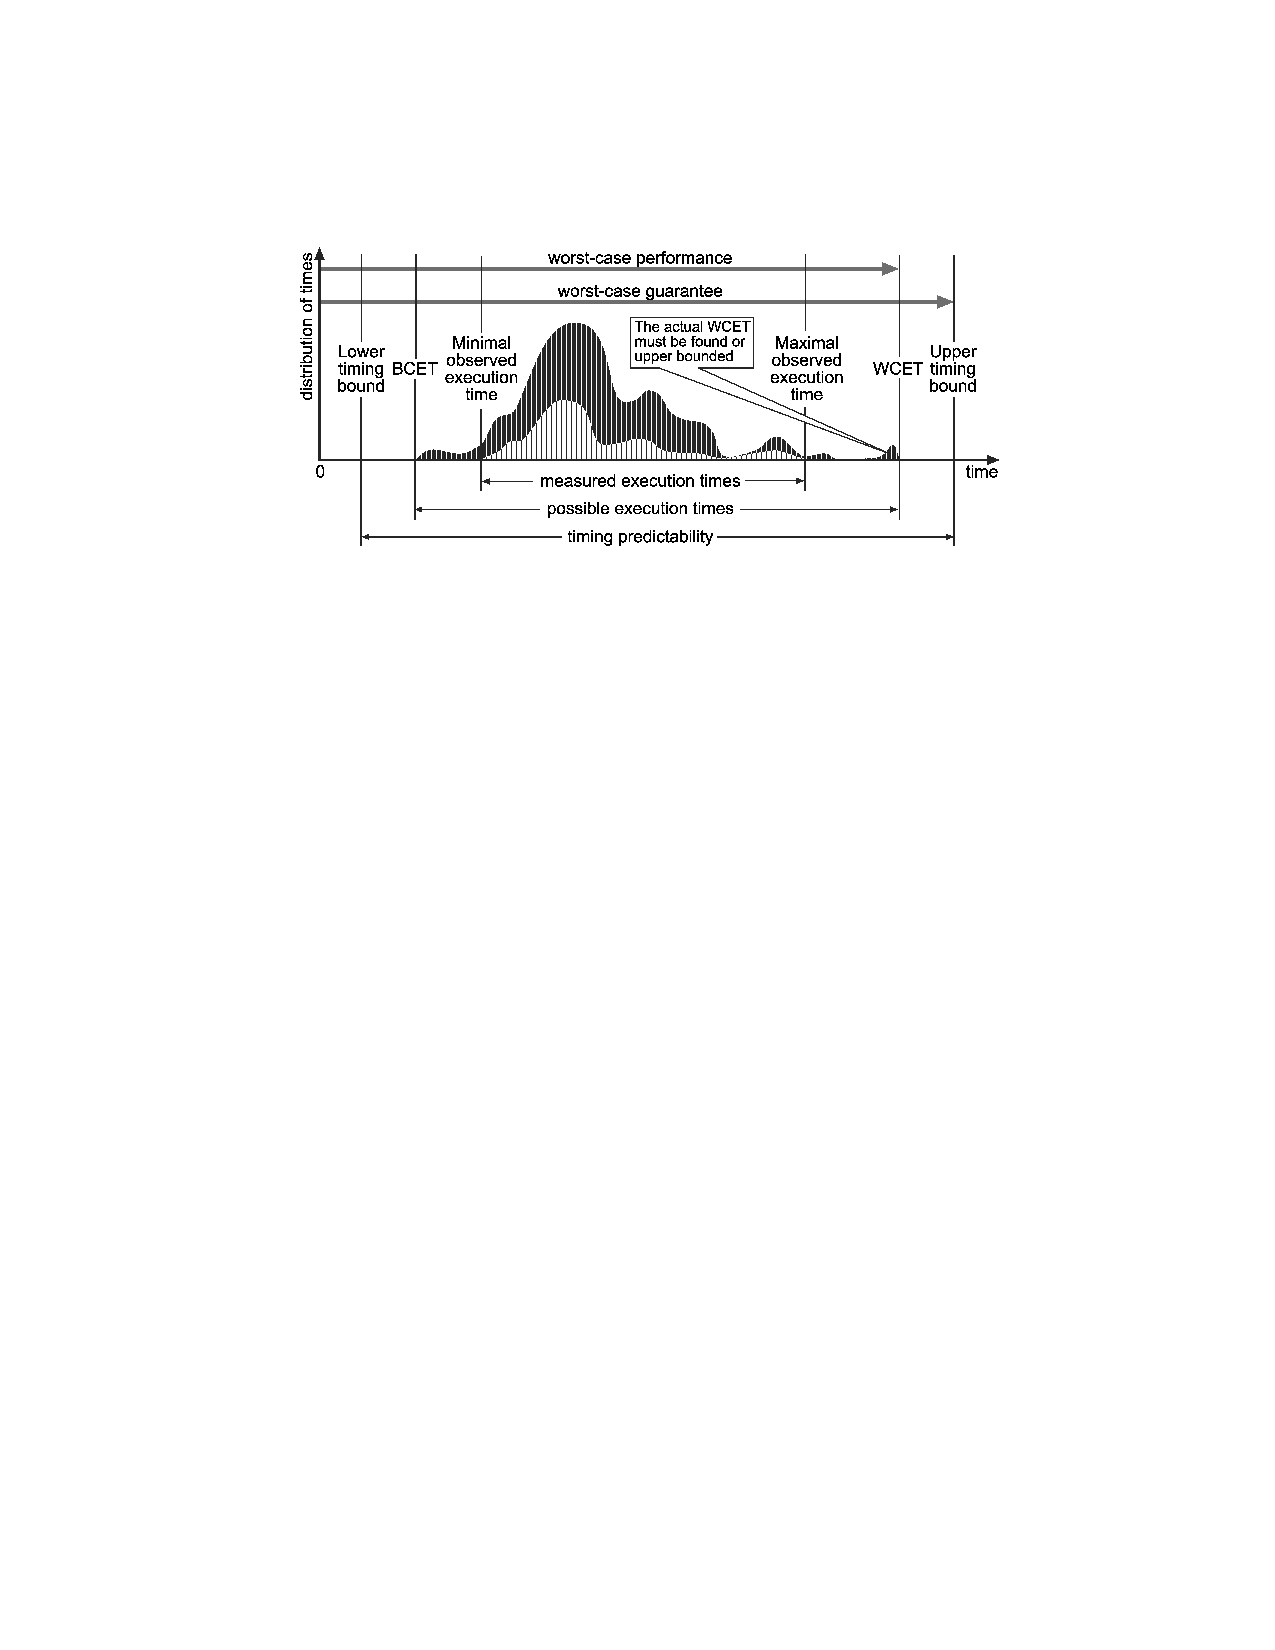
\includegraphics{figs/program_executiontimes.pdf}
  \end{center}
  \vspace{-3mm}
  \caption{Program Execution Times~\cite{wilhelm-survey-paper}}
  \label{fig:program_execution_times}
\end{figure}

It highlights several key issues that are important to understanding program execution time.
First, the \emph{observable execution times} may not observe all \emph{possible execution times}.
This is important because far too often we rely on testing and end-to-end measurement to determine the WCET.
This will, in general, overestimate the BCET and underestimate the WCET, and is not safe when timing must be guaranteed. 
Second, it is often difficult to determine the \emph{actual} WCET, thus the worst case guarantee that is given is usually a bound on the WCET.    
The goal of the WCET analysis is to obtain a \textit{safe} and \textit{precise} bound on the WCET of a program~\cite{Wilhelm2008survey}. 
\textit{Safe} means that the execution time will never exceed the bounded time. 
\textit{Precise} means that the bounded time is as close to the absolute WCET as possible. 

Several factors contribute to the difficulties of a safe and precise WCET analysis.
In general, it is impossible to obtain the upper bounds on execution times for programs because programs are not guaranteed to terminate.  
Real-time systems use a restricted form of programming to ensure an execution time upper bound.
Recursion is often not allowed or must be explicitly bounded, as are the iteration counts of loops. 
Despite that, algorithms contain input dependent program paths that complicate analysis.    
The worst case program path depends on the worst-case input, which in general, is not known or hard to derive.    

Along with complications from the software structure, the execution time variance exhibited by the underlying architecture further complicates analysis.   
A conventional microprocessor executes a sequence of instructions from an instruction set. 
Each instruction in the instruction set changes the state of the processor in a well-defined way.
The microprocessor provides a strong guarantee about this behavior: a sequence of instructions \emph{always} changes the processor state in the sequential order of the instructions.        
For speed, however, modern microprocessors rarely execute the instructions strictly in sequence. 
Instead, pipelines, caches, write buffers, and out-of-order execution reorder and overlap operations while preserving the illusion of sequential execution.  
This causes the execution time of even the same sequence of instructions to fluctuate, depending on the underlying execution of its instructions.
To illustrate this, we show in figure~\ref{fig:simple_code_timing_issues} a code segment with a simple control structure and a static loop bound.

%predictability -   
  % C code example
  % modern architecture improvements
\begin{wrapfigure}{r}{0.45\textwidth}
  \vspace{-20pt}
  \begin{center}
    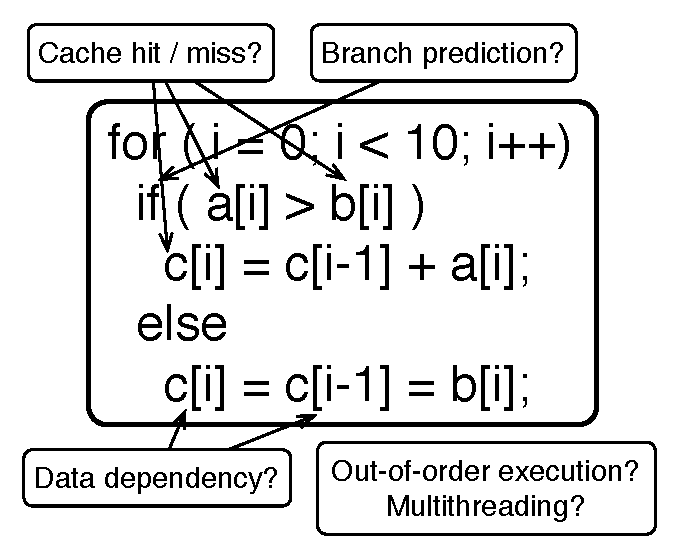
\includegraphics[scale=.6]{figs/simple_code_timing_issues}
  \end{center}
  \vspace{-10pt}
  \caption{Simple Loop Timing Issues}
  \label{fig:simple_code_timing_issues}
  \vspace{-10pt}
\end{wrapfigure}

Even with a simple software structure, several situations can arise from the execution on the underlying architecture. 
Each array access in the code is compiled into a memory access.
Whether the memory access hits or misses the cache has huge implications on program execution time.
The \emph{if} statement is usually compiled to a conditional branch, and the outcome of the branch predictor could easily affect the execution time of the program.
%Furthermore, the speculatively executed instructions could modify the cache state which can cause future memory accesses to delay.        
Superscalar architectures can execute instructions out-of-order, thus data-dependencies in this code may or may not stall, depending on the memory accesses and how much loop unrolling is done by the compiler/architecture.   

Further complications arise as architectures become increasingly parallel with multiprocessing techniques such as multicore and multithreading.
These techniques allow the architecture to inherently handle concurrency, but can easily introduce temporal interference even between logically independent behaviors.
For example, in a multicore machine with shared caches, the processes running on one core can affect the timing of processes on another core even when there is no communication between these processes.
Similarly, Simultaneous Multithreading ~\cite{Eggers97simultaneousmultithreading} architectures share a wide-issue superscalar pipeline across multiple hardware threads.
Instructions are dispatched from all threads simultaneously using scoreboaring mechanisms.
However, the contention for pipeline resources between threads can easily vary the execution time of a particular thread. 

% On the other hand, symmetric multiprocessing (SMP) techniques use multiple processing units connected with an on-chip communication interconnect such as a bus or network-on-chip.
% SMP exploits thread-level parallelism by designating a thread to a different processing unit.
% While this removes temporal interference caused by sharing pipeline resources between multiple threads, temporal interference is reintroduced at the on-chip communication interconnect.
% For instance, sharing the same off-chip memory between processing units requires arbitration and coherence, which results in temporal interference.
% In fact, any sharing of resources such as busses, memories, switches, buffers, and I/O devices can result in temporal interference.
\begin{wrapfigure}{r}{0.5\textwidth}
  \vspace{-20pt}
  \begin{center}
    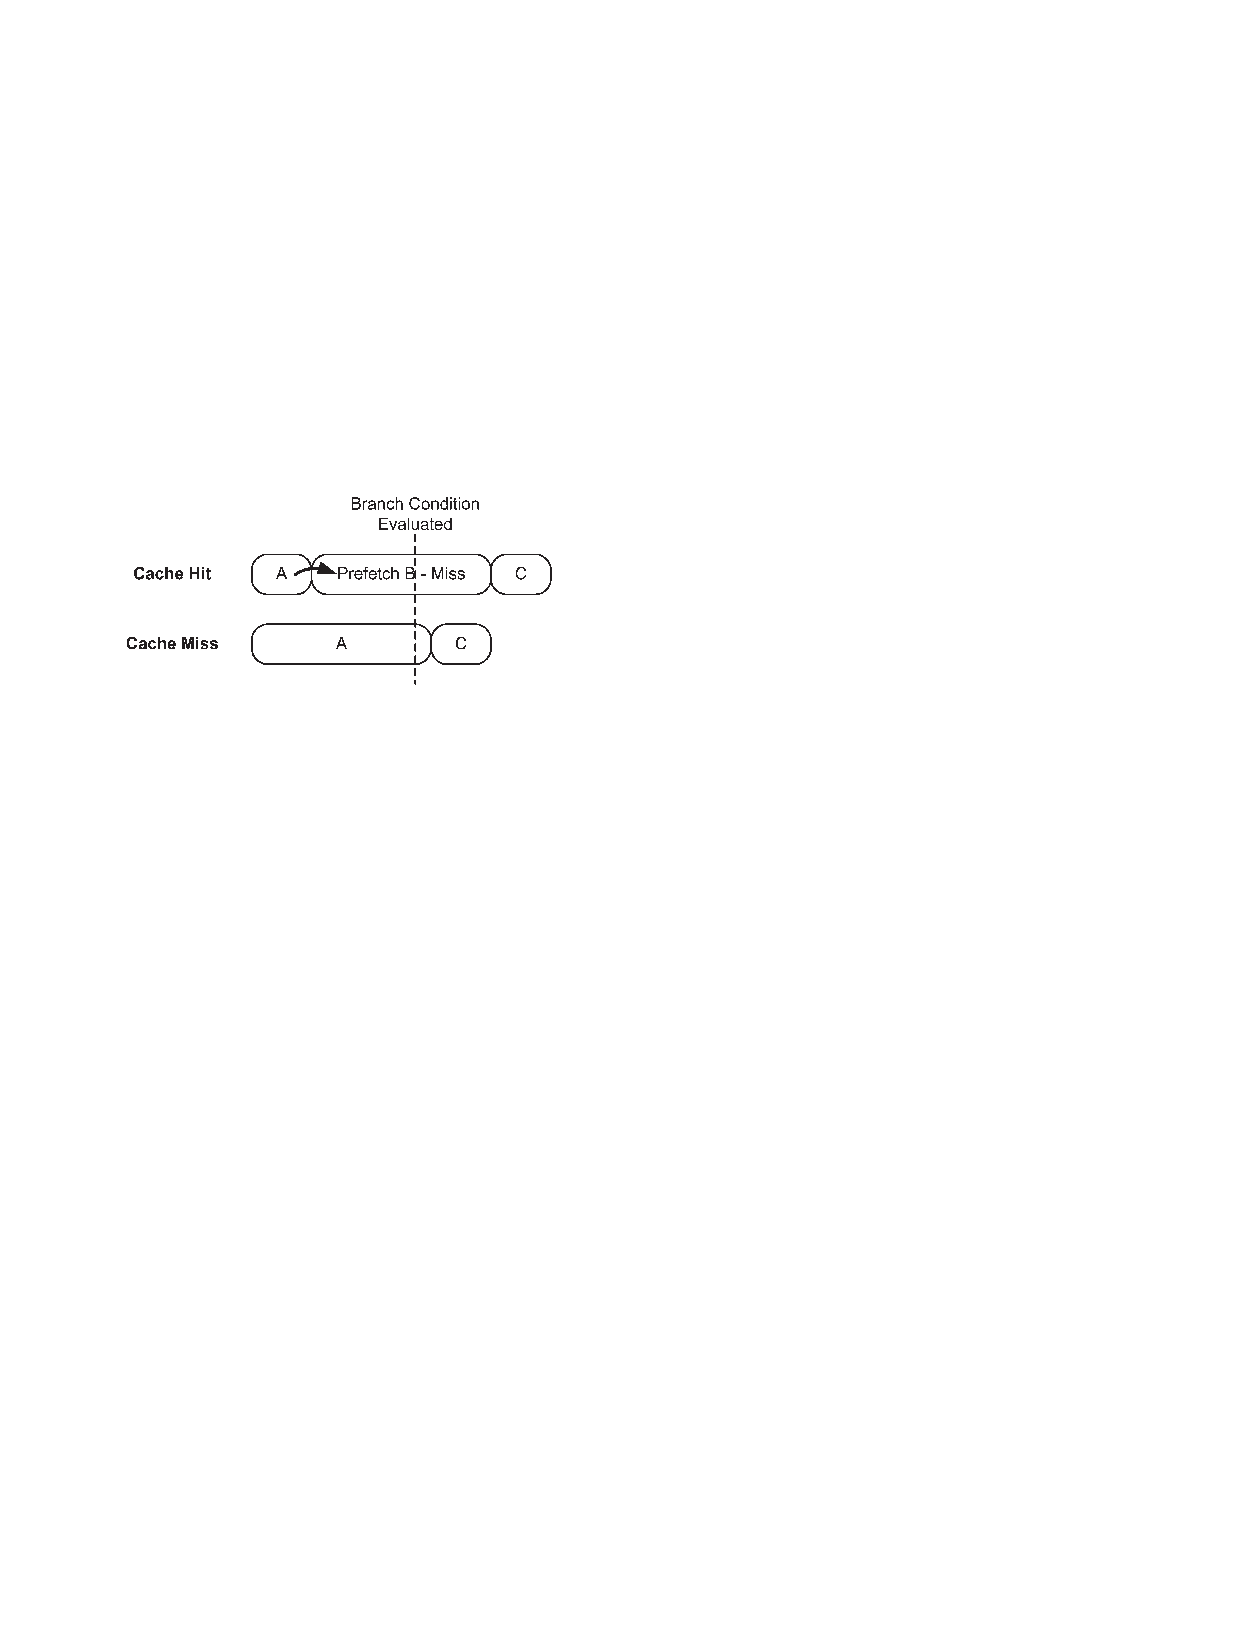
\includegraphics{figs/speculation_anomaly}
  \end{center}
  \vspace{-10pt}
  \caption{Timing anomaly cause by speculation~\cite{Reineke06adefinition}}
  \label{fig:speculation_anomaly}
  \vspace{-10pt}
\end{wrapfigure}
The common misconception is that at least a \emph{safe} upper bound on the execution time can be easily determined by assuming the worse case in unknown situations.
This is not true because dynamic processors can exhibit \emph{timing anomalies}~\cite{Reineke06adefinition,Lundqvist1999}, situations where a local worst-case does not entail the global worst-case.
Reineke et al.~\cite{Reineke06adefinition} illustrates this with the example in figure~\ref{fig:speculation_anomaly}.
In this example, a mispredicted branch results in unnecessary instruction fetching that destroys the cache state. 
However, if the first instruction being fetched is a cache miss, the correct branch condition will be computed before the fetch, and no speculatively executed instruction will destroy the cache state. 
This example shows that simply assume a cache miss (local worst-case) will not always lead to the global worst-case execution time.    

The increasing complexity of architectures leads to the conclusion that the usefulness of the results of WCET analysis strongly depends on the architecture of the employed processor~\cite{Heckmann2003processor}.
Modern processors employ features that improve average performance at the expense of worst-case performance, creating a large variation in execution time from the processor. 
These features are controlled and manage completely in hardware, not explicitly exposed to the software.
As a result, decrypting the state of the processor to obtain reasonable execution time estimates is often extremely difficult, if not impossible, on modern architectures.   

\section{Precision Timed Machines}
In this thesis we introduce the design and implementation of PREcision Timed (PRET) machines~\cite{Edwards2007PRETcase}. 

places timing predictability and composability as its first class citizen.   

We aim to present architectures
%proposed a paradigm shift in the design of computer architectures, focusing on timing predictability instead of average-case performance.
%provide better wcet
%use thread-interleaved pipline and dram controller
%ISA extensions
%needed for autosar etc

With designs being pushed to higher and higher levels of abstraction, we need lower levels to provide robust, non brittle fundamentals in which we can reason about timing guarantees.


As Wilhelm et al. \cite{wilhelm2009} quoted:
\begin{quote} \textit{
  ``The applicability of the AUTOSAR idea depends on availability of
  architectures on which software composition does not lead to
  unpredictable timing behavior.''
}
\end{quote}

% \begin{itemize}
% \item \emph{Low jitter} -- Small variance in execution time for a given code block, enabling a tight WCET bound.
% \item \emph{Continuous}~\cite{Henzinger2008} -- small changes in the input result in small changes in the output.
% \item Precise timing control, which is the ability to control temporal
%   properties in the architecture.
% \item Reasonable performance, or else someone could use a processor
%   from 20 years ago to achieve some of the effects above.
% \item Repeatable performance, mainly that the same execution yields
%   the same output. Including execution time. (\textcolor{red}{This
%     needs careful defining... what counts as input and what counts as
%     output?})
% \item Composability - The ability to compose two tasks without
%   interference. This is an extremely important property to preserve
%   because when we design systems, we want to design larger systems
%   from smaller components. We want to test those smaller systems
%   separately, then compose them and still have those tested properties
%   hold true. 
% \end{itemize}
% Through this, enable evaluation on the effects and implications on the composition, communication and synchronization of software components or tasks on a predictable architecture.

The remaining chapters are organized as follows. 
Chapter~\ref{chapter:pret} explains the architecture of PRET including the \thdint pipeline and memory hierarchy, Chapter~\ref{chapter:ptarm}, Chapter~\ref{chapter:app}, Chapter~\ref{chapter:related}, Chapter~\ref{chapter:summary}.


